\documentclass[addpoints]{exam}
\usepackage[utf8]{inputenc}
\usepackage[portuguese]{babel}
\usepackage[LGRgreek]{mathastext}
\usepackage{graphicx,graphics}
\usepackage{hyperref}
%\usepackage{framed}
\usepackage{multirow}
\usepackage{booktabs}
\usepackage{pdfpages} 

\footer{}{\thepage}{}

%%% INÍCIO DOS COMANDOS ACRESCENTADOS NO NETBOOK %%%%%%%%%%%%%%%%%%%
\newcommand*{\renameenviron}[1]{%
  \expandafter\let\csname exam-#1\expandafter\endcsname
      \csname #1\endcsname
  \expandafter\let\csname endexam-#1\expandafter\endcsname
      \csname end#1\endcsname
  \expandafter\let\csname #1\endcsname\relax
  \expandafter\let\csname end#1\endcsname\relax
}
\renameenviron{framed}
\renameenviron{shaded}
\renameenviron{leftbar}
%%% FIM DOS COMANDOS ACRESCENTADOS NO NETBOOK %%%%%%%%%%%%%%%%%%%
\usepackage{framed}

\renewcommand{\arraystretch}{1.3}
%\setlength{\tabcolsep}{pt}
 
\pointpoints{ponto}{pontos}
\bonuspointpoints{ponto extra}{pontos extra}
 
\totalformat{Pregunta \thequestion: \totalpoints pontos}
 
\chqword{Pregunta}
\chpgword{Página}
\chpword{Pontos}
\chbpword{Pontos extra}
\chsword{Pontos obtidos}
\chtword{Total}

\hqword{Questão}
\hpgword{Página}
\hpword{Pontos}
\hsword{Pontos obtidos}
\htword{Total}

 
\begin{document}
 
\large

\begin{center}
\Large
\textbf{Laboratório de Eletrônica Básica II – EE641}
\end{center}

\large
\vspace{2mm}

\noindent\textbf{Profs.:} Dr. Eduardo T. Costa\hfill \textbf{Turma 01/2022} \\
\textbf{PED:} Mathias Scroccaro Costa \hfill %\textbf{e-mail:} mathias.scroccaro@gmail.com

\normalsize
 
\vspace{5mm}
 

 
\noindent\makebox[0.72\textwidth]{Nome: \enspace\hrulefill}
\hfill
\makebox[0.2\textwidth]{RA: \enspace\hrulefill}

\vspace{5mm}

\noindent\makebox[0.72\textwidth]{Nome: \enspace\hrulefill}
\hfill
\makebox[0.2\textwidth]{RA: \enspace\hrulefill}

\vspace{5mm}

\noindent\makebox[0.72\textwidth]{Nome: \enspace\hrulefill}
\hfill
\makebox[0.2\textwidth]{RA: \enspace\hrulefill}


%\begin{center}
%\gradetable[h][questions]
%\end{center}

\vspace{2mm}


\begin{center}
\large
\textbf{AMPLIFICADOR DE INSTRUMENTAÇÃO}
\normalsize
\end{center}

\begin{questions}

\section*{Amplificador de Instrumentação}

\question Monte o circuito amplificador de instrumentação em \textbf{placa furada padrão}, conforme o esquemático da Figura \ref{cir:1}. Conside Rf = 50 k$\Omega$ e Rg = 10 k$\Omega$. Conecte o nó ``DAC'' à saída do circuito gerador de sinais de ECG. Não esqueça de disponibilizar \textit{pinheads} machos, para a alocação de \textit{mini jumpers}, pois serão fundamentais ao testar o circuito.

\begin{figure}[h!]
\begin{center}
\includegraphics[width=0.9\textwidth]{imagens/ecg.pdf}
\end{center}
\caption{Circuito amplificador de instrumentação.}
\label{cir:1}
\end{figure}

\pagebreak

\begin{parts}

\part \label{part:1} Utilizando um gerador de sinais, insira uma forma de onda senoidal com 0,1 V de amplitude e frequência de 10 Hz sobre o nó ``mini jumper \#1''. Com auxílio de um osciloscópio, monitore através do canal 1 o gerador de sinais; e com o canal 2 a forma de onda observada em ``Vout''. Utilizando o recurso ``Measure'', mostre no display do osciloscópio a tensão de pico a pico de ambos os canais. Salve os sinais vistos no osciloscópio, em uma única figura, imprima-a e anexe-a ao relatório. A amplitude da forma de onda observada é coerente com o esperado? 

\pagebreak

\part Ainda com o \textit{setup} montado do item (\ref{part:1}), verifique na prática a frequência de corte do filtro passa-altas:
\begin{subparts}
\subpart \label{subpart:1} Para frequência inicial de 10 Hz, anote a tensão de pico a pico vista em ``Vout'';
\subpart Gradualmente, diminua a frequência do gerador de sinais até o momento em que a tensão de pico a pico vista em ``Vout'' é -3 dB do valor do item (\ref{subpart:1}).
\subpart Salve a forma de onda de entrada (mini jumper \#1) e saída (Vout) em que ocorre a frequência de corte, em uma única figura, imprima-a e anexe-a ao relatório. 
\end{subparts} 

\pagebreak

\part (PÓS EXPERIMENTO) Quais as três topologias de amplificadores operacionais que estão presentes neste circuito?
\begin{framed}
\vspace{5cm}
\end{framed}

\part (PÓS EXPERIMENTO) Encontre a função algébrica de ganho do circuito Amplificador de Instrumentação G(V+,V-,Rg,Rf). Considere o nó Vref = 0 V.
\begin{framed}
\vspace{6cm}
\end{framed}

\part (PÓS EXPERIMENTO) Cite três vantagens da configuração Amplificador de Instrumentação. Qual o problema da implementação discreta deste circuito?
\begin{framed}
\vspace{6cm}
\end{framed} 

\pagebreak

\part (PÓS EXPERIMENTO) O circuito montado pode ser representado pela malha de controle mostrada abaixo. Baseado nesta representação, quais os valores de G e H(s)? Encontre a função de transferência total do sistema, substituindo os valores de G e H(s).
\begin{framed}
\begin{center}
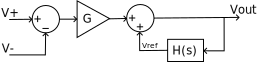
\includegraphics[width=0.5\textwidth]{imagens/control_system.pdf}
\end{center}
\vspace{10cm}
\end{framed}


\end{parts}





\end{questions}



\end{document}
